\documentclass[10pt,a4paper]{article}
\usepackage[margin=25mm]{geometry}
\usepackage{amsmath,amssymb,amsthm,booktabs,array}
\usepackage[T1]{fontenc}
\usepackage{lmodern}
\usepackage{alltt,longtable}
\usepackage{xurl}
\usepackage[hidelinks]{hyperref}
\usepackage{microtype}
\usepackage{tikz}
\setlength{\parskip}{4pt}
\setlength{\parindent}{1em}
\setlength{\emergencystretch}{2em}
\renewcommand{\arraystretch}{1.13}
\renewcommand{\topfraction}{.9}
\renewcommand{\bottomfraction}{.6}
\renewcommand{\textfraction}{.08}
\renewcommand{\floatpagefraction}{.75}
\setcounter{topnumber}{3}
\setcounter{totalnumber}{4}
\newtheorem{theorem}{Theorem}
\newtheorem{lemma}[theorem]{Lemma}
\newtheorem{proposition}[theorem]{Proposition}
\newtheorem{corollary}[theorem]{Corollary}
\theoremstyle{definition}
\newtheorem{definition}[theorem]{Definition}
\theoremstyle{remark}
\newtheorem{remark}[theorem]{Remark}
\newcommand{\Z}{\mathbb Z}
\newcommand{\Halo}{\operatorname{Halo}}
\newcommand{\Hc}{H_{\mathrm c}}
\newcommand{\Hh}{H_{\mathrm h}}
\newcommand{\lean}[1]{\texttt{#1}}
\title{Heesch numbers and maximal coronas of small polyforms\newline
with certificates and a Lean-verified SAT encoding}
\author{Tatsuhiko Takimoto\\\small Independent researcher}
\date{Version 2.1, 23 October 2026}
\begin{document}
\maketitle
\begin{abstract}
For a fixed selection of 3,964 shapes from Kaplan's tables of unmarked
polyforms, we give 6,574 corona witnesses and 5,019 upper-bound proofs
accepted by drat-trim. A Lean~4 soundness theorem for the SAT encoding
covers the square, hexagonal and triangular grids; six theorem statements
are accepted in six kernel runs using five implementations. A finite
comparison connects all 5,019 checked CNFs to the Lean definition, and a
separately written encoding agrees on every value. The proof checking
and file comparison remain external to Lean.
We also count maximal coronas for 22 selected shapes, distinguishing
$\Hh$ (holes permitted in the outermost layer) from $\Hc$ (no holes).
Two implementations agree completely on 28 of the 30 shape--variant
combinations; the other two totals are available from one implementation
only. In the fully compared cases every fixed extendable inner part has
more than one outer completion, while exactly six $\Hh$ cases and four
$\Hc$ cases have a unique inner part. Inner enumeration has checked DRAT
exhaustion proofs in those 28 cases; the outer counts rely on agreement
of separate counting implementations sharing the same encoding and
geometric specification. A further, restricted search of 3,442
polyominoes with 20--28 cells yields no example with finite $\Hh=4$.
\end{abstract}

\section{Introduction}
\label{sec:intro}
A shape that does not tile the plane may still be surrounded by copies of
itself. Its Heesch number is the largest number of complete layers
(coronas) of congruent copies that can be placed around it. The problem of
which values occur goes back to Heesch~\cite{Heesch}; Mann's survey
\cite{Mann} describes its history and gives edge-marked hexapillars with
Heesch numbers 4 and 5, Fontaine~\cite{Fontaine} found an infinite family of figures with
Heesch number~2, and Ba\v{s}i\'c~\cite{Basic21} constructed a figure with Heesch
number~6. Kaplan's recent account~\cite{Kaplan25} describes the present
state of the problem in the plane; related questions have been studied in
the hyperbolic plane~\cite{Maiti} and in three dimensions~\cite{Basic26}.

Computation has been central to this work. Mann and Thomas computed
Heesch numbers of edge-marked polyforms~\cite{MannThomas}. Kaplan
\cite{Kaplan} encoded the existence of all coronas up to a given order as
a single SAT problem, distinguished the hole-free Heesch number $\Hc$ from
the number $\Hh$ in which the outermost corona may contain holes, and
computed both values for unmarked polyominoes, polyhexes and polyiamonds,
publishing the tables, the shapes and the software~\cite{heeschsat}. The
question studied here, the definitions of coronas and of $\Hc,\Hh$, the
idea of a SAT search over all layers at once, and every reference value
we compare with are taken from Kaplan's work. The Heesch challenge of
Layr-Labs/Eigen~\cite{Layr} already attaches checkable certificates to
Heesch numbers: it checks corona witnesses geometrically, regenerates CNFs
from a shape and a layer count and compares their digests, converts DRAT
proofs to LRAT and checks them with the verified checker
cake\_lpr~\cite{cakelpr}, and records verified upper-bound proofs for
individual shapes with high Heesch numbers. At the commit we consulted,
its documentation states that an external review of the correspondence
between the geometry and the CNF is still pending. Its census of 3,943
known non-tilers is the same size as the complete, small-size portion of
our selection; the additional selected shapes have high Heesch numbers.

A DRAT proof certifies that one particular CNF formula is unsatisfiable.
Whether that formula expresses ``there is no $K$-layer corona'' is a
separate question, which is usually answered by the correctness of the
program that generated it. This article addresses that question for one
encoding, on all three grids, with a theorem proved in Lean, and connects
the theorem to the files that were actually checked. Its contributions
are:
\begin{enumerate}
\item for a fixed, hash-identified selection of 3,964 shapes from
Kaplan's tables, a lower-bound witness and an upper-bound certificate for
every value of $\Hc$ and $\Hh$, with all 5,019 proofs accepted by
drat-trim~\cite{dratTrim} (Sections~\ref{sec:certificates}
and~\ref{sec:results});
\item a Lean~4 statement and proof that the encoding is sound on the
square, hexagonal and triangular grids, for every order of the
at-most-one counters and every admissible set of hole-blocking clauses
(Sections~\ref{sec:encoding} and~\ref{sec:lean});
\item a finite comparison showing that each of the 5,019 checked CNF files
is, up to renaming and reordering, the Lean-defined CNF
(Section~\ref{sec:bridge});
\item counts of maximal coronas and of their extendable prefixes for the
22 shapes attaining the largest $\Hh$ in each selected grid range, with
separate implementations agreeing completely in 28 of 30 shape--variant
combinations (Section~\ref{sec:counts});
\item a documented search of a fixed set of 3,442 polyominoes with 20--28
cells, with no finite-$\Hh=4$ example obtained
(Section~\ref{sec:search}).
\end{enumerate}
Formal verification of SAT encodings and of reductions from geometry to
SAT has clear precedents: Codel, Avigad and Heule verified encodings,
including the sequential counter, in Lean~\cite{CodelThesis,CAH}; Holliday,
Norman, Pacuit and Zahedian proved in Lean that the existence of a
voting rule yields a model of their CNF~\cite{Holliday}; Subercaseaux,
Nawrocki, Gallicchio, Codel, Carneiro and Heule verified the reduction
behind the empty hexagon number and connected it to a cake\_lpr
check~\cite{EmptyHex}. Our formalization applies this approach to the
coronas, holes and candidate placements of the Heesch problem on three
grids. Section~\ref{sec:scope} compares the guarantees in more detail.

\section{What is claimed, and on what basis}
\label{sec:status}
Table~\ref{tab:status} lists the claims and the kind of evidence behind
each. Who ran which check, when, and with which tool versions is recorded
in the verification record that accompanies this article
(\mbox{\texttt{VERIFICATION-RECORD.md}}). The article has not undergone
human expert review.

{\small
\begin{longtable}{@{}>{\raggedright\arraybackslash}p{.34\linewidth}
>{\raggedright\arraybackslash}p{.41\linewidth}
>{\raggedright\arraybackslash}p{.19\linewidth}@{}}
\caption{Claims and their basis. Finite checks use programs that are not
formally verified.}\label{tab:status}\\
\toprule
Claim & Basis & Range\\
\midrule
\endfirsthead
\multicolumn{3}{@{}l}{\textit{Table~\thetable\ continued}}\\
\toprule Claim & Basis & Range\\\midrule
\endhead
\bottomrule\endfoot
\multicolumn{3}{@{}l}{\emph{Lean proof}}\\
CNF soundness (Theorem~\ref{thm:sound}) & Six theorems; standard axioms
\lean{propext}, \lean{Classical.choice}, \lean{Quot.sound}; six kernel
runs (five implementations) & Three grids, all $K\geq1$, counter orders
and valid blocks\\
Square-grid instance equals the earlier square-only definition & Lean
proof outside the Comparator statement, same axioms & All arguments\\
\midrule
\multicolumn{3}{@{}l}{\emph{Prose}}\\
Truncation and $\Hh-1\leq\Hc\leq\Hh$; counting conventions and
minimality (Proposition~\ref{prop:minimal}) &
Lemma~\ref{lem:trunc}; the arguments in Section~\ref{sec:counts} &
Stated domains\\
Disc criteria used in counting: hole tests suffice for inner layers;
Euler-characteristic tests for the outer $\Hc$ layer &
Elementary topology (Section~\ref{sec:enum}) & Hexagonal and triangular
outer layers; all inner layers\\
Empty-block UNSAT excludes every (P0)--(P3) patch, without disc conditions &
Consequence of the proof outline of Theorem~\ref{thm:sound}, stronger than
its Lean statement & Empty block list\\
\midrule
\multicolumn{3}{@{}l}{\emph{AI review}}\\*
Lean definitions express the geometry and encoding faithfully &
Independent reading against the specification and Kaplan;
``faithful with caveats'' & Statement file\\
\midrule
\multicolumn{3}{@{}l}{\emph{Finite computation}}\\*
Upper bounds and file correspondence & drat-trim accepts 5,019 proofs;
Python transcriptions match 64 Lean outputs, then all 5,019 CNFs up to
renaming and reordering & Table~\ref{tab:bridge}\\
Lower bounds and independently encoded values & Two geometric checkers
accept 6,574 witnesses; second encoding agrees on all values, without
proof logs & 3,964 shapes\\
Maximal-corona prefix enumeration & Coordinate-wise agreement; checked
DRAT exhaustion of the enumeration CNFs on both sides (these CNFs are
outside the Lean theorem and the file comparison); every solution checked
geometrically & 28 combinations;
\#315 prefixes agree without checked DRAT\\
Outer completions and total counts & Two separate counting implementations
agree per inner part; no proof certificate for the outer counts &
28 totals agree; two \#315 totals from one side\\
Restricted search & SAT screening and explicit periodic tilings; 14
solver cross-checks and two sampled DRAT checks & 3,442 shapes;
Table~\ref{tab:search}\\
\midrule
Not claimed & Exhaustiveness beyond the listed inputs; off-grid
placements; Lean-internal UNSAT or file-comparison proofs; formally
verified counting & \\
\end{longtable}}


The end-to-end statement for the tabulated values rests on: (1) the correctness of the Lean kernel and Mathlib;
(2) the faithfulness of the Lean definitions to the intended geometry;
(3) the correctness of drat-trim;
(4) file identity established through SHA-256, and the correctness of the
Python transcriptions and file-comparison programs; and
(5) for the lower bounds, the correctness of the geometric witness checkers.

\section{Coronas and Heesch numbers on three grids}
\label{sec:defs}
We follow Kaplan~\cite[Sections~2.1 and~4]{Kaplan}. Points of $\Z^2$
index cells. A \emph{grid} specifies which points are cells, when two
cells \emph{touch} (share at least one point of the plane), when they
share an edge, which affine maps $x\mapsto Mx+w$ are allowed congruences,
and what a \emph{pinch vertex} is. Table~\ref{tab:grids} gives the three
grids. On the hexagonal grid the point $(x,y)$ is the centre $xv+yw$ of a
regular hexagon, with $v=(1,0)$ and $w=(1/2,\sqrt3/2)$. The triangular
grid uses the same coordinates: a point is a cell (a triangle with that
centroid) if $x\equiv y\equiv0$ or $x\equiv y\equiv1\pmod 3$; points
with $x\equiv y\equiv2\pmod3$ are vertices. The black cell $(x,y)$ has
vertices $(x-1,y+2)$, $(x-1,y-1)$, $(x+2,y-1)$, and the grey cell
$(x,y)$ has vertices $(x+1,y-2)$, $(x+1,y+1)$, $(x-2,y+1)$. The twelve
hexagonal orientations are $A^iB^j$ ($0\leq i<6$, $j\in\{0,1\}$) with
\[
A=\begin{pmatrix}0&-1\\1&1\end{pmatrix},\qquad
B=\begin{pmatrix}1&1\\0&-1\end{pmatrix},
\]
acting by $(x,y)\mapsto(ax+by,\,cx+dy)$ for the matrix
$\bigl(\begin{smallmatrix}a&b\\c&d\end{smallmatrix}\bigr)$.

\begin{table}[!htbp]
\centering\small
\begin{tabular}{@{}>{\raggedright\arraybackslash}p{.15\linewidth}
>{\raggedright\arraybackslash}p{.22\linewidth}
>{\raggedright\arraybackslash}p{.22\linewidth}
>{\raggedright\arraybackslash}p{.33\linewidth}@{}}
\toprule
& Square & Hexagonal & Triangular\\
\midrule
Cells & all of $\Z^2$ & all of $\Z^2$ & $x\equiv y\equiv0$ or
$x\equiv y\equiv1\pmod 3$\\
Touch & 8 neighbours $N_8$ & 6 offsets $(\pm1,0)$, $(0,\pm1)$, $\pm(1,-1)$
& share $\geq1$ vertex (12 neighbours)\\
Share an edge & 4 neighbours $N_4$ & same as touch & share 2 vertices (3
neighbours)\\
Orientations & 4 rotations, 4 reflections & $A^iB^j$ (12) & $A^iB^j$
(12)\\
Translations $w$ & $\Z^2$ & $\Z^2$ & $M(2,2)+w\equiv(2,2)\pmod 3$\\
Distance $d$ & $\max(|a|,|b|)$ & $\max(|a|,|b|,|a+b|)$ & $0$ for the same
cell; otherwise $1+\min$ of the hexagonal distance of $(u-u')/3$ over
vertices $u$, $u'$ of the two cells\\
Pinch vertex & two diagonal cells of four & none & incident cells form
$\geq2$ runs around a vertex\\
Scan box for (F) & $\pm K$ & $\pm K$ & $\pm4K$\\
\bottomrule
\end{tabular}
\caption{The three grids. $(a,b)$ is the difference of two cells; the
distance from a set $T_0$ is the minimum over its cells. On the triangular
grid the translation condition says that vertices are mapped to
vertices; it selects one residue class of $w$ modulo $3\Z^2$ for each
matrix.}
\label{tab:grids}
\end{table}

A \emph{shape} $S$ is a finite set of cells, a \emph{copy} of $S$ is its
image under an allowed congruence, and $\Halo(X)$ is the set of cells not
in $X$ that touch a cell of $X$. A finite set $P$ of cells has a
\emph{hole} if some cell outside $P$ lies in a finite component of the
complement of $P$ under edge adjacency. We call $P$ a \emph{disc} if
(a)~$P$ is connected under edge adjacency, (b)~$P$ has no hole, and
(c)~$P$ has no pinch vertex. For finite unions of cells these three
conditions describe a closed topological disc; the formal statement
below uses the combinatorial conditions themselves.

\begin{samepage}
\begin{definition}[Coronas]
\label{def:corona}
Let $k\geq0$. A \emph{$k$-corona} of $S$ is a finite set of copies of $S$,
each with a layer number in $\{0,\dots,k\}$, such that, writing $P_j$ for
the union of the copies of layer at most $j$,
\begin{itemize}
\item[(P0)] the only copy of layer $0$ is $S$ itself;
\item[(P1)] distinct copies are disjoint;
\item[(P2)] $\Halo(P_j)\subseteq P_{j+1}$ for $j<k$;
\item[(P3)] every copy of layer $j\geq1$ has a cell in $\Halo(P_{j-1})$.
\end{itemize}
It is an \emph{$\Hh$-corona} if $P_0,\dots,P_{k-1}$ are discs, and an
\emph{$\Hc$-corona} if $P_0,\dots,P_k$ are discs. The numbers $\Hc(S)$ and
$\Hh(S)$ are the largest $k$ for which an $\Hc$-corona, respectively an
$\Hh$-corona, with $k$ layers exists.
\end{definition}
\end{samepage}

All copies lie on the fixed grid, as in Kaplan's SAT
setting~\cite[Section~3]{Kaplan}. Reported Heesch values concern
hole-free disc-shaped polyforms. If the central shape has a hole, the
$P_0$ condition excludes every positive-layer $\Hh$-corona and even a
zero-layer $\Hc$-corona; such shapes are omitted from Kaplan's files used
here.

\begin{lemma}
\label{lem:trunc}
\textup{(i)} If $S$ has an $\Hh$-corona \textup{(}$\Hc$-corona\textup{)}
with $k$ layers, it has one with $k'$ layers for every $k'\leq k$.
\textup{(ii)} $\Hh(S)-1\leq\Hc(S)\leq\Hh(S)$.
\end{lemma}
\begin{proof}
(i) Keep the copies of layer at most $k'$. The sets $P_0,\dots,P_{k'}$ do
not change, so (P0)--(P3) and the disc conditions for $j\leq k'$ are
inherited. (ii) An $\Hc$-corona is an $\Hh$-corona. Truncating an
$\Hh$-corona with $k$ layers to $k-1$ layers gives an $\Hc$-corona, since
$P_0,\dots,P_{k-1}$ are discs.
\end{proof}

Consequently, the nonexistence of an $\Hh$-corona with $K$ layers gives
$\Hc\leq\Hh\leq K-1$, and the nonexistence of an $\Hc$-corona with $K$
layers gives $\Hc\leq K-1$.

\section{The SAT encoding}
\label{sec:encoding}
The input is a shape $S$, a grid, and a number of layers $K\geq1$. Write
$T_0=S$ and let $d(c)$ be the distance of a cell $c$ from $T_0$ in the
touching graph (Table~\ref{tab:grids}).

\begin{lemma}[Distance bound]
\label{lem:A}
In a $k$-corona, every cell $c$ with $d(c)\leq j\leq k$ lies in $P_j$.
Hence every cell of a copy of layer $j$ has $d\geq j$.
\end{lemma}
\begin{proof}
By induction on $j$, using $P_j\supseteq P_{j-1}\cup\Halo(P_{j-1})$,
which is (P2). A cell with $d<j$ then lies in $P_{j-1}$, so by (P1) it is
not in a copy of layer $j$.
\end{proof}

\paragraph{Pruning.}
Let $R_0=T_0$. For $j=1,\dots,K$, a copy $p$ of $S$ disjoint from $T_0$
is a candidate at layer $j$ if its halo meets $R_{j-1}$. A candidate is
given the interval of layers $\Lambda(p)=[\mathrm{lo}(p),\mathrm{hi}(p)]$,
where $\mathrm{lo}(p)$ is the first $j$ at which it qualifies and
$\mathrm{hi}(p)=\min(K,\min_{c\in p}d(c))$, and $R_j$ is $R_{j-1}$
together with the cells of all candidates allowed at layer $j$. Then,
for $j<K$, a pair $(p,j)$ is kept only if $\Halo(p)\setminus T_0\subseteq
R_{j+1}$, the sets $R_j$ are recomputed from the remaining pairs, and the
touching and halo tests are repeated until nothing changes. By
Lemma~\ref{lem:A}, (P2) and (P3), every copy of a genuine corona survives
with its layer: the cells it touches lie in $R_{j-1}$ and the copies
covering its halo lie in $R_{j+1}$.

\paragraph{Variables.}
$t_{p,j}$ for $j\in\Lambda(p)$ (copy $p$ is used at layer $j$);
$y_{c,j}$ for $1\leq j\leq K$ and $c\in R_j\setminus T_0$ (cell $c$ is
covered by layers $\leq j$); auxiliary variables of the at-most-one
counters; and, if needed, one fresh variable $b$.

\paragraph{Clauses.}
\begin{itemize}
\item[(F)] $y_{c,d(c)}$ for every cell with $1\leq d(c)\leq K$
(Lemma~\ref{lem:A}). If some such $c$ is not in $R_{d(c)}$, the clauses
$b$ and $\neg b$ are added instead of the missing unit.
\item[(Y1)] $y_{c,j-1}\to y_{c,j}$.
\item[(Y2)] $y_{c,j}\to y_{c,j-1}\vee\bigvee\{t_{p,j}: c\in p\}$, the
first disjunct omitted when $y_{c,j-1}$ does not exist.
\item[(B)] $t_{p,j}\to y_{c,j}$ for $c\in p$.
\item[(C)] For each cell $c$, at most one of the variables $t_{p,j}$ with
$c\in p$ is true, by Sinz's sequential counter~\cite{Sinz}: for inputs
$x_1,\dots,x_m$ and auxiliary $s_1,\dots,s_{m-1}$, the clauses
$x_1\to s_1$; $x_a\to s_a$, $s_{a-1}\to s_a$, $x_a\to\neg s_{a-1}$ for
$1<a<m$; and $x_m\to\neg s_{m-1}$. This gives (P1) and a single layer per
copy.
\item[(D)] For $j<K$: $t_{p,j}\to y_{c,j+1}$ for $c\in\Halo(p)\setminus
T_0$; if $y_{c,j+1}$ does not exist, the clause is $\neg t_{p,j}$. This
gives (P2).
\item[(E)] For $j\geq2$ and $p$ not touching $T_0$:
$t_{p,j}\to\bigvee\{y_{c,j-1}: c\in\Halo(p)\setminus T_0\}$. This gives
(P3); for $j=1$ it holds by construction.
\end{itemize}
The order in which the inputs of each counter are listed is a free
choice. We write $\mathrm{ord}$ for this choice and
$F_{\mathrm{ord}}(S,K,\mathcal B)$ for the resulting CNF with a list
$\mathcal B$ of hole blocks.

\paragraph{Hole blocks.}
A satisfying assignment may describe a patch whose layer $P_j$ has a
hole, which an $\Hh$-corona forbids for $j\leq K-1$ and an $\Hc$-corona
for $j\leq K$. A \emph{block} $(j,H,E)$ consists of a level $j$, a set of
cells $H$ and a list $E$ of copies with layers. It is \emph{valid} for a
maximal level $L$ if $1\leq j\leq L$, $H$ is nonempty and consists of
cells, every copy in $E$ has layer at most $j$, and every edge neighbour
of $H$ outside $H$ lies in a copy of $E$. It adds the clause
\[
\textstyle\bigvee_{(p,l)\in E}\neg t_{p,l}\ \vee\ \bigvee_{c\in H}y_{c,j},
\]
in which the entry $(0,T_0)$ contributes no literal, and each
$y_{c,j}$ that does not exist is omitted. Such a cell cannot belong to
$P_j$. The block is skipped if $H$ meets $T_0$ or if some other entry of
$E$ is not a variable. The clause can be empty, which is still sound for
a valid block.
Kaplan's hole clauses~\cite[Section~3.2]{Kaplan} contain only the
negative literals; the positive literals added here keep the
assignments in which other copies fill $H$, so these clauses are weaker.
If every copy in $E$ is used and no cell of $H$ is covered by layers
$\leq j$, then $H$ is cut off from the rest of the complement of $P_j$,
so $P_j$ has a hole. On the triangular grid the requirement that $H$
consist of cells matters: a non-cell point has no edge neighbours, so
without it a block on such a point would produce an empty clause.

\begin{theorem}[Soundness]
\label{thm:sound}
Let the grid be square, hexagonal or triangular, let $S$ be a finite set
of points, $K\geq1$, let $\mathrm{ord}$ list each counter's inputs in some
permutation, and let every block in $\mathcal B$ be valid for maximal
level $K-1$ \textup{(}resp.\ $K$\textup{)}. If
$F_{\mathrm{ord}}(S,K,\mathcal B)$ is unsatisfiable, then $S$ has no
$\Hh$-corona \textup{(}resp.\ $\Hc$-corona\textup{)} with $K$ layers.
\end{theorem}
\begin{proof}[Proof outline]
Given such a corona, set $t_{p,j}$ true when $p$ is a copy of layer $j$,
$y_{c,j}$ true when $c\in P_j$, and each counter variable $s_a$ true when
one of the first $a$ inputs is. Pruning keeps every genuine copy at its
layer, so the variables exist and (F) needs no fresh variable. Clauses
(Y1), (Y2), (B) and (D) follow from the definitions and (P2), (C) from
(P1), (E) from (P3), and each block clause from the disc condition of
$P_j$. The formal proof is described in Section~\ref{sec:lean}.
\end{proof}

With an empty block list, the same assignment in the proof outline
satisfies the CNF for every patch obeying (P0)--(P3), without any disc
conditions: no block clause remains to use them. Thus UNSAT excludes all
such patches. This is a prose consequence of the proof, not one of the
six formal statements in Lean (Table~\ref{tab:status}). The value computation solves
$K=1,2,\dots$ without hole conditions on the outer layer until the first
unsatisfiable $K$, which gives $\Hh=K-1$; when a solution has a hole in
an inner layer, a block is added and the problem is solved again. If the
witness for $\Hh$ has a hole in its outer layer, the problem with $K=\Hh$
and the $\Hc$ condition decides between $\Hc=\Hh$ and $\Hc=\Hh-1$
(Lemma~\ref{lem:trunc}). Hole blocks can occur in intermediate SAT
calls during the value search; the final upper-bound certificates use
blocks only for $\Hc$, as shown in Table~\ref{tab:certs}.

\section{The Lean formalization}
\label{sec:lean}
The formal statement imports only Mathlib~\cite{Mathlib} and was written before the
proof, directly from the mathematical description above. A structure
\lean{Grid} carries the fields of Table~\ref{tab:grids}: a predicate
\lean{isCell}, the relations \lean{Touch} and \lean{EdgeAdj}, a predicate
\lean{Pinch}, the list of orientation matrices, the translation test
\lean{transOk}, and three computable helpers (the list of touching cells,
the distance $d$, and the box scanned by (F)). The three grids are the
values \lean{squareGrid}, \lean{hexGrid} and \lean{triGrid}; the twelve
hexagonal matrices are computed inside the statement as products
$A^iB^j$. Copies, halos, holes, discs and the predicates
\lean{IsCoronaHh} and \lean{IsCoronaHc} are defined once for an arbitrary
grid, following Definition~\ref{def:corona}. A hole cell is required to
satisfy \lean{isCell}; otherwise every non-cell point of the triangular
grid would be a finite component of the complement and every patch would
have a hole. The pruning and the CNF are computable functions
\lean{candidates} and \lean{cnfOrd}, a CNF being a list of lists of
integer literals, with literal $0$ interpreted as false. The six theorems
\lean{hh\_sound\_square}, \lean{hc\_sound\_square}, \lean{hh\_sound\_hex},
\lean{hc\_sound\_hex}, \lean{hh\_sound\_tri} and \lean{hc\_sound\_tri}
state Theorem~\ref{thm:sound}. The triangular $\Hh$ case reads (in ASCII
notation; the source uses the corresponding Unicode symbols):
{\small
\begin{alltt}
theorem hh_sound_tri (ord : Cell -> List Int -> List Int)
    (hord : forall c g, (ord c g).Perm g)
    (S : List Cell) (K : Nat) (hK : 1 <= K) (blocks : List HoleBlock)
    (hblocks : forall b, b \(\in\) blocks -> b.Valid triGrid (K - 1))
    (hunsat : Not (Satisfiable (cnfOrd triGrid ord S K blocks))) :
    Not (exists tiles : Tiles, IsCoronaHh triGrid S.toFinset K tiles)
\end{alltt}}
\noindent Here \lean{Satisfiable F} means that some assignment
$\sigma:\mathbb N\to\{\mathrm{true},\mathrm{false}\}$ makes a literal of
every clause true, and \lean{HoleBlock.Valid} is the validity condition of
Section~\ref{sec:encoding}.

\paragraph{Proof.}
The proof constructs the satisfying assignment of the proof outline of
Theorem~\ref{thm:sound}. All grid-dependent facts are collected in nine
properties (touching agrees with the neighbour list and is symmetric,
touching cells are cells, edge adjacency is symmetric, four properties of
the distance, and allowed congruences map non-cells to non-cells), proved
separately for each grid. Lemma~\ref{lem:A} then follows for every grid
from the property that the distance decreases by one along some touching
step. On the triangular grid this step property is the main geometric
lemma: from a minimal pair of vertices one moves along an edge of the
vertex lattice, and the triangle on that edge touches the current cell
and is one step closer. The survival of genuine copies under pruning is
proved by an invariant of each refinement round; it uses neither that the
iteration reaches a fixed point nor that its bound on the number of
rounds suffices. The proof files have 1,837 lines.

\paragraph{Checks.}
Comparator, in paranoid mode, checks that the proof proves exactly the
six statements of the statement file and replays them in six kernel runs
using five implementations: the Lean kernel in paranoid and default mode,
lean4lean, nanoda, con-leche and con-ron; all six runs accept
\cite{Comparator,Lean4Lean,OtherKernels}. \lean{\#print axioms} reports only
\lean{propext}, \lean{Classical.choice} and \lean{Quot.sound}, and the
files contain no \lean{sorry}, \lean{native\_decide} or new axiom. The
environment is Lean~4.35.0~\cite{Lean4} with Mathlib~v4.35.0~\cite{Mathlib}. A further theorem,
outside the Comparator statement, shows that \lean{cnfOrd squareGrid}
equals an earlier square-only definition for all arguments, so results
established for the earlier definition carry over.

\paragraph{Reading of the statement.}
An independent AI reader compared the statement with the mathematical
description and with Sections~2.1 and~4 of~\cite{Kaplan}, before seeing
any proof. It checked the hexagonal and triangular cells, neighbours,
orientations and translation classes, compared both distance formulas
with breadth-first search, checked the pinch test on all 64 occupancy
patterns around a triangular vertex, and confirmed on small examples that
the definitions are not vacuous. Its verdict was ``faithful with
caveats''. The caveats are part of the scope: the theorems accept any
finite set of points as $S$, including sets that are not polyforms (the
theorems remain true for such inputs but then say nothing about
polyforms); copies are placed on the fixed grid; and the link between a
checked DIMACS file and \lean{cnfOrd} lies outside the statement.

\section{Certificates}
\label{sec:certificates}
\paragraph{Shapes.}
The shapes and reference values are read from Kaplan's published files
\cite{Kaplan}, two lines per shape (cell coordinates and the values
$\Hc,\Hh$). The 22 files that contain the selected shapes, and the
files searched to complete the selection, are identified by their SHA-256
hashes in the verification record. For each grid, Kaplan publishes all
hole-free non-tilers up to a size and, for larger sizes, only the shapes with $\Hh$ above a
threshold. Our selection is listed in Table~\ref{tab:values}.

\paragraph{Lower bounds.}
For each shape we give a witness for $\Hh$ and one for $\Hc$, combined into
a single witness when the same patch serves both (1,354 shapes), in total
6,574 witnesses. A witness lists every copy with its layer and absolute
cells. Two separately written checkers, neither of which uses the
encoding, test congruence of every copy, (P0)--(P3),
the disc conditions (a)--(c) for the layers required by $\Hc$ or $\Hh$,
and that $k$ equals the claimed value. Both accept all 6,574 witnesses.

\paragraph{Upper bounds.}
For each shape, one certificate states that there is no $\Hh$-corona with
$K=\Hh+1$ layers; all 3,964 of these use an empty block list, so the prose consequence of the soundness proof excludes every
$K$-layer patch satisfying (P0)--(P3), even without disc conditions. For the 1,055 shapes
with $\Hc<\Hh$, a second certificate states that there is no $\Hc$-corona
with $K=\Hc+1$ layers; these carry 13,287 hole blocks in total. Each
certificate records the CNF (SHA-256, size, numbers of variables and
clauses) and a proof of unsatisfiability. The proofs were produced by
CaDiCaL~1.5.3~\cite{CaDiCaL} (4,998 binary DRAT proofs),
Glucose~4.1~\cite{Glucose} (16 DRUP proofs) and
Lingeling~\cite{Lingeling} (5 text DRAT proofs), all through
python-sat~1.9.dev17~\cite{PySAT}, and all
5,019 are accepted by drat-trim~\cite{dratTrim}. The CNFs and proofs are
not archived: the largest single proof has 7,175,887,914 bytes. The CNFs
are regenerated deterministically: all 5,019 agree with the recorded
hashes and sizes. Proofs are regenerated by rerunning the recorded
solver. Proof-hash reproduction has been tested in four large cases:
five-layer $\Hh$ bounds for two 15-cell polyhexes, a 13-cell polyhex and
a 20-cell polyiamond. Each regenerated proof agrees with the recorded
hash and is accepted by drat-trim, with at most 3.01\,GB of memory.

\paragraph{Second encoding.}
A second encoding, written from the mathematical description of the
encoding without access to the first implementation and solved with
the same SAT solvers through python-sat, recomputes all bounds. Its
encoding code is independent; the mathematical specification and SAT
solvers are shared. It
agrees with the first encoding and with Kaplan on $\Hc$ and $\Hh$ for all
3,964 shapes; the 6,574 witnesses, read as assignments, satisfy all of
its clauses; and all 5,019 upper-bound instances are unsatisfiable. This second
computation did not produce proof logs; it is an independent check of the
values, not a second certificate.

\begin{table}[!htbp]
\centering\small
\begin{tabular}{@{}lrrrrrrr@{}}
\toprule
& & & \multicolumn{2}{c}{Certificates} & Accepted by & &
Largest CNF\\
\cmidrule(lr){4-5}
Grid & Shapes & Witnesses & $\Hh$ & $\Hc$ & drat-trim & Blocks &
(clauses)\\
\midrule
Square & 1,616 & 2,766 & 1,616 & 460 & 2,076 & 7,267 & 2,926,850\\
Hexagonal & 437 & 808 & 437 & 100 & 537 & 2,126 & 6,588,816\\
Triangular & 1,911 & 3,000 & 1,911 & 495 & 2,406 & 3,894 & 5,869,683\\
\midrule
Total & 3,964 & 6,574 & 3,964 & 1,055 & 5,019 & 13,287 & \\
\bottomrule
\end{tabular}
\caption{Witnesses and upper-bound certificates. Blocks occur only in
the $\Hc$ certificates. The largest CNFs are a four-layer bound for a
17-omino, and five-layer bounds for a 15-hex and a 20-iamond.}
\label{tab:certs}
\end{table}

\begin{table}[!htbp]
\centering\small
\setlength{\tabcolsep}{4.2pt}
\begin{tabular}{@{}llrrrrrrrrrr@{}}
\toprule
Grid & Cells (selection) & Shapes & \multicolumn{9}{c}{Number of shapes
with $(\Hc,\Hh)=$}\\
\cmidrule(l){4-12}
& & & (0,0) & (0,1) & (1,1) & (1,2) & (2,2) & (2,3) & (3,3) & (3,4) &
(4,4)\\
\midrule
Square & 7 (all) & 3 & & 1 & 2 & & & & & & \\
& 8 (all) & 20 & & 6 & 13 & 1 & & & & & \\
& 9 (all) & 198 & 36 & 39 & 118 & 4 & 1 & & & & \\
& 10 (all) & 1,390 & 355 & 392 & 628 & 14 & 1 & & & & \\
& 11--19 ($\Hh=3$) & 5 & & & & & & 3 & 2 & & \\
\midrule
Hexagonal & 6 (all) & 4 & & & 3 & & 1 & & & & \\
& 7 (all) & 37 & 4 & 1 & 18 & 7 & 5 & 1 & 1 & & \\
& 8 (all) & 381 & 37 & 33 & 220 & 44 & 40 & 4 & 3 & & \\
& 9--16 ($\Hh=4$) & 15 & & & & & & & & 10 & 5\\
\midrule
Triangular & 7 (all) & 1 & & & 1 & & & & & & \\
& 9 (all) & 20 & 7 & 4 & 9 & & & & & & \\
& 10 (all) & 103 & 33 & 11 & 48 & 7 & 3 & & & 1 & \\
& 11 (all) & 594 & 117 & 119 & 327 & 19 & 11 & & 1 & & \\
& 12 (all) & 1,192 & 495 & 331 & 361 & 3 & 1 & & 1 & & \\
& 13--24 ($\Hh=4$) & 1 & & & & & & & & & 1\\
\midrule
Total & & 3,964 & 1,084 & 937 & 1,748 & 99 & 63 & 8 & 8 & 11 & 6\\
\bottomrule
\end{tabular}
\caption{The certified Heesch numbers. ``All'' means every shape in
Kaplan's file of hole-free non-tilers with that number of cells. The polyominoes
with $\Hh=3$ have 11, 13, 17, 17 and 17 cells (one with $(2,3)$ each for
11 and 13 cells; $(2,3)$, $(3,3)$, $(3,3)$ for 17 cells). The polyhexes
with $\Hh=4$ have 10 (1), 11 (6), 12 (2), 13 (2), 15 (2) and 16 (2) cells.
The polyiamonds with $\Hh=4$ are a 10-iamond with $(\Hc,\Hh)=(3,4)$
and a 20-iamond with $(4,4)$. There are no non-tiling 8-iamonds in
Kaplan's census (his Table~5). Kaplan's files for
$n\geq11$ cells (square), $n\geq9$ (hexagonal) and $n\geq13$
(triangular) list only shapes above a threshold of $\Hh$; the selected
shapes are all shapes in these files with the stated $\Hh$, the largest
value occurring in each group of files.}
\label{tab:values}
\end{table}

\section{From the checked files to the Lean CNF}
\label{sec:bridge}
Theorem~\ref{thm:sound} is about \lean{cnfOrd}; drat-trim checked DIMACS
files written by a separate program. Two CNFs $F$ and $F'$ are
\emph{equivalent up to renaming} if there is a bijection $\pi$ of the
variables such that applying $\pi$ (without changing signs) to $F$ gives
the same multiset of clauses as $F'$, each clause compared as a multiset
of literals. Such $F$ and $F'$ are equisatisfiable. For each of the 5,019
certificates we compared the checked file with
\lean{cnfOrd G ord S K blocks} for the recorded grid, shape, $K$ and
blocks, as follows.
\begin{enumerate}
\item The checked file is regenerated and its SHA-256 hash and size are
compared with the certificate record (all 5,019 agree).
\item The Lean definition of \lean{cnfOrd} is transcribed into Python
without reading the source of the generating program. The transcription
uses two Python transcriptions, one for the square grid and one for
the hexagonal and triangular grids. They are validated against Lean's
own evaluation: 64 outputs (30 square and 34 hexagonal/triangular,
including hole blocks, the fresh variable $b$, and default and reversed
counter orders) agree byte for byte. For the square grid, the comparison
is with the earlier square-only definition; the Lean equality theorem
outside the Comparator statement identifies it with
\lean{cnfOrd squareGrid}.
\item From the checked file, the input order of every at-most-one counter
and a bijection of variables are recovered; the recovered orders are
checked to be permutations.
\item The checked file, renamed by the bijection, and the transcription
with the recovered orders are compared clause by clause as multisets,
read by two different DIMACS parsers, without merging duplicates,
simplifying or flipping signs.
\item Every block is checked against \lean{HoleBlock.Valid}; on the
triangular grid all 6,922 hole points are cells.
\end{enumerate}
The two programs differ in where they number the fresh variable $b$
(after the cell variables, or after the counter variables) and in the
order of literals within clauses; both differences are absorbed by the
bijection and by comparing clauses as multisets. The comparison was
performed for all 5,019 CNFs (Table~\ref{tab:bridge}), with no mismatch
and no undecided case. No compared clause contains literal $0$;
the DIMACS clause terminators are removed before comparing literals.
This distinguishes the file convention from Lean's false-literal
convention.

\begin{table}[!htbp]
\centering\small
\begin{tabular}{@{}lrrrrl@{}}
\toprule
Grid & CNFs & Variables & Clauses & Blocks & CNFs by $K$ ($K=1,2,3,4,5$)\\
\midrule
Square & 2,076 & 45,711,523 & 178,454,670 & 7,267 & 829, 1,218, 24, 5, 0\\
Hexagonal & 537 & 39,687,752 & 168,537,425 & 2,126 & 75, 326, 102, 19, 15\\
Triangular & 2,406 & 48,014,519 & 191,702,313 & 3,894 & 1,117, 1,240, 44, 3, 2\\
\midrule
Total & 5,019 & 133,413,794 & 538,694,408 & 13,287 & \\
\bottomrule
\end{tabular}
\caption{The file comparison. All 5,019 checked CNFs are equivalent up
to renaming to \lean{cnfOrd} with the recovered counter order, and all
blocks are valid. Variables and clauses are summed over the CNFs.}
\label{tab:bridge}
\end{table}

\begin{corollary}
\label{cor:chain}
Assume (1) the correctness of the Lean kernel and Mathlib;
(2) the faithfulness of the Lean definitions to the intended geometry;
(3) the correctness of drat-trim;
(4) file identity established through SHA-256, and the correctness of the
Python transcriptions and file-comparison programs; and
(5) for the lower bounds, the correctness of the geometric witness checkers. Then for each shape in
Table~\ref{tab:values}, there is no $\Hh$-corona with $\Hh+1$ layers and
no $\Hc$-corona with $\Hc+1$ layers, so the upper bounds hold; the
witnesses give the lower bounds.
\end{corollary}
\begin{proof}
By the comparison, each checked CNF is equisatisfiable with
\lean{cnfOrd} for a permutation order and valid blocks, so
Theorem~\ref{thm:sound} applies; Lemma~\ref{lem:trunc} turns the
nonexistence of $K$-layer coronas into the bound $K-1$. For a shape
with $\Hc=\Hh$, the $\Hh$ certificate also bounds $\Hc$.
\end{proof}

\section{Results}
\label{sec:results}
Table~\ref{tab:values} lists the selection and the distribution of the
certified values. In every one of the 3,964 shapes, the certified pair
$(\Hc,\Hh)$ equals the pair in Kaplan's file. Within the selection,
every shape satisfies $\Hc\in\{\Hh-1,\Hh\}$, as Lemma~\ref{lem:trunc}
requires. The largest values are $\Hh=3$ for polyominoes and $\Hh=4$ for
polyhexes and polyiamonds; the five polyhexes with $\Hc=\Hh=4$ (one
11-hex, one 13-hex, two 15-hexes and one 16-hex) and the 20-iamond with
$\Hc=\Hh=4$ have the largest certified hole-free values. The other
polyiamond with $\Hh=4$ is the 10-iamond with $\Hc=3$.


\section{Counting maximal coronas}
\label{sec:counts}
A \emph{maximal $\Hh$-corona} of $S$ is an $\Hh$-corona of $S$ with
exactly $k=\Hh(S)$ layers, and a \emph{maximal $\Hc$-corona} is an
$\Hc$-corona with the same number $k$ of layers; ``maximal'' refers to the
number of layers, not to inclusion.
The 22 shapes in Table~\ref{tab:counts} attain the largest $\Hh$ in
each grid range selected here: five polyominoes with $\Hh=3$, fifteen
polyhexes with $\Hh=4$, and two polyiamonds with $\Hh=4$. The polyhex
range stops at 16 cells: Kaplan's published Table~4 has an additional
17-cell example, which is outside our inputs. For each shape we count
$\Hh$-coronas at $k=\Hh(S)$; for the eight shapes with $\Hc=\Hh$ we
also count $\Hc$-coronas at the same $k$.

\subsection{Objects, symmetry and prefixes}
A configuration is a finite set of pairs $(j,p)$, where $p$ is the cell
set of a copy and $j$ its layer. The counting conventions are:
\begin{enumerate}
\item Two configurations are identified exactly when a grid congruence
fixing the central cell set $S$ maps one to the other. This group is the
central stabilizer $G(S)$.
\item Copies are cell sets: their ordering, multiple congruences giving
the same copy, and assignments to the SAT auxiliary variables are not
counted.
\item Layer labels are retained. They can also be recovered from the
set of copies: once $P_{j-1}$ is known, every copy outside it that touches
it must have layer $j$, since a higher-layer copy would overlap the
halo already covered by $P_j$. Induction recovers all layers.
\item Extra copies beyond a corona are not permitted. Each copy in
layer $j$ must touch $P_{j-1}$, as required by (P3).
\end{enumerate}
The raw count distinguishes all coordinates; the orbit count divides
only by the action of $G(S)$. A finite calculation gives $|G(S)|=1$ for
all 22 central shapes, so the two counts coincide.

A prefix of depth $j$ is the restriction of a maximal $k$-corona to
layers at most $j$. Write $N_j$ for the number of distinct such prefixes.
These are precisely the prefixes that extend to $k$ layers, not all
$j$-coronas. An \emph{inner part} is a prefix of depth $k-1$.

\begin{proposition}[Minimality of the counted configurations]
\label{prop:minimal}
No two distinct $k$-coronas satisfying (P0)--(P3), considered as sets of
layered copies, contain one another. The same holds for their prefixes
of a fixed depth when both prefixes extend to $k$ layers.
\end{proposition}
\begin{proof}
Suppose $Q\subsetneq Q'$ and take an extra copy of $Q'$ of smallest
layer $i$. Both configurations have the same $P_{i-1}$. By (P3) that
copy contains a cell of $\Halo(P_{i-1})$, already covered by a layer-$i$
copy of $Q$ by (P2). It therefore overlaps a different copy of $Q'$,
contradicting (P1). The same argument works for a prefix, since (P2)
through the preceding layer is inherited from its extension.
\end{proof}

\subsection{Enumeration and completion counts}
\label{sec:enum}
The computation separates inner parts from the last layer. At $K=k$,
a SAT solver enumerates projections onto the inner placement variables.
Every solution found is a complete $k$-layer configuration and is checked
by the geometric witness checker. For the inner layers $P_1,\dots,P_{k-1}$
the disc conditions reduce to the absence of holes. By (P2), $P_j$
contains $P_{j-1}\cup\Halo(P_{j-1})$; a cell touching $P_{j-1}$ is joined
to it by edge-adjacent cells around a common vertex, all in this union,
and every copy of layer $j$ is edge-connected and meets $\Halo(P_{j-1})$.
By induction from $P_0=S$, each $P_j$ is edge-connected. In an edge-connected set, a pinch
vertex of the square or triangular grid encloses a cell of the
complement and so produces a hole, and the hexagonal grid has no pinch
vertices. When a solution has a hole in an inner layer, a hole clause is
added as in Section~\ref{sec:encoding}. A blocking clause
containing the negations of the selected inner placements removes just
that prefix, by Proposition~\ref{prop:minimal}; this is a prose argument,
not an extension of the Lean theorem. A second implementation instead
blocks the complete signed assignment of all inner placement variables,
so it does not depend on that minimality argument.

For a fixed inner part with union $U=P_{k-1}$, an outer layer is an exact
cover of $\Halo(U)$ by copies disjoint from $U$ and from each other.
Disjointness is tested on the whole cell sets, including cells outside
the halo. Each selected copy covers at least one halo cell, so (P3)
excludes surplus copies. For $\Hc$ the completed union must also be a
disc. Summing the number of outer completions over the distinct inner
parts gives $N_k$.

Two separate implementations enumerate the inner projections and count
the outer completions, sharing the CNF encoding, hole-clause generator,
grid definitions and geometric witness checker. The second independently
generates outer candidates and uses a different projected blocking rule.
For $\Hc$ it uses direct disc tests on the square grid. On the
hexagonal grid the completed union is edge-connected and has no pinch
vertex, so it is a disc exactly when its Euler characteristic is $1$;
on the triangular grid the same test is combined with boundary
conditions that exclude pinch vertices.
The first uses direct geometric hole pruning with memoization. Agreement
is checked per inner configuration in cell coordinates, not just in
the final sum.

In 28 of 30 combinations, the prefix sets, all prefix counts, every
inner part's completion count and the total agree. Both implementations
have drat-trim-checked exhaustion proofs for those inner enumerations.
Such a proof certifies that the final enumeration CNF, consisting of the
base clauses, the inner hole clauses and all blocking clauses, is
unsatisfiable. The enumeration CNFs are produced by the same generator as
the certified upper-bound CNFs, but they are covered neither by the Lean
theorem, which has no blocking clauses, nor by the file comparison of
Section~\ref{sec:bridge}, which concerns the 5,019 upper-bound CNFs.
That no further extendable inner part exists therefore also rests on
the shared generator, the validity of its hole clauses and, for the
first implementation, Proposition~\ref{prop:minimal}.
The outer completion counts themselves have no proof certificate and
are not formalized in Lean. They are exact finite counts corroborated
by the separate implementations. Further checks enumerate complete
$k$-coronas directly by SAT, without separating the outer layer: nine
combinations in the first implementation, each ending in a
drat-trim-checked unsatisfiable call, and six in the second. The second
implementation also recounts the outer layers of 12 inner parts, in
eight combinations, by backtracking without memoization. All these
checks agree with Table~\ref{tab:counts}.

For 15-hex \#315 both implementations enumerate the same 979 $\Hh$
and 79 $\Hc$ inner parts and the same shallower prefixes, but neither
has a checked DRAT exhaustion proof for them. Its totals in
Table~\ref{tab:counts} are from the second counter only. The first
implementation completed the outer counts of 26 of the 79 $\Hc$ inner
parts before stopping. Of these, 22 agree with the second
implementation; the other four were flagged as invalid by the first
implementation's own check on its memoized hole tests. It did not finish
the $\Hh$ outer count; the three per-inner-part values it reported agree
with the second implementation. These counting
exhaustion checks are distinct from the checked five-layer upper-bound
certificate for this shape in Table~\ref{tab:certs}.

{\small\setlength{\tabcolsep}{4pt}
\begin{longtable}{@{}llcrrrr@{}}
\caption{Maximal-corona counts. Shape identifiers are zero-based row
indices in Kaplan's indicated size/threshold files. Here $k=\Hh(S)$;
$N_j$ counts prefixes extendable to a $k$-corona of the indicated variant,
and the last column is $N_k$. A dash marks $j=k$, already in the last
column. Every central stabilizer is trivial, so raw and orbit counts
coincide. All entries agree between the two implementations except the
$\dagger$ totals, available from one only; their prefix counts agree but
have no checked DRAT exhaustion proof.}\label{tab:counts}\\
\toprule
Shape & $(\Hc,\Hh)$ & Variant & $N_1$ & $N_2$ & $N_3$ & $N_k$\\
\midrule\endfirsthead
\multicolumn{7}{@{}l}{\textit{Table~\thetable\ continued}}\\
\toprule Shape & $(\Hc,\Hh)$ & Variant & $N_1$ & $N_2$ & $N_3$ & $N_k$\\
\midrule\endhead
\bottomrule\endfoot
11-omino \#2 & $(2,3)$ & $\Hh$ & 1 & 1 & -- & 1,250\\
13-omino \#50 & $(2,3)$ & $\Hh$ & 1 & 1 & -- & 594\\
17-omino \#43 & $(3,3)$ & $\Hh$ & 1 & 1 & -- & 430\\
17-omino \#43 & $(3,3)$ & $\Hc$ & 1 & 1 & -- & 28\\
17-omino \#192 & $(3,3)$ & $\Hh$ & 2 & 4 & -- & 1,168\\
17-omino \#192 & $(3,3)$ & $\Hc$ & 1 & 1 & -- & 2\\
17-omino \#521 & $(2,3)$ & $\Hh$ & 1 & 2 & -- & 20,160\\
10-hex \#13 & $(3,4)$ & $\Hh$ & 3 & 3 & 9 & 768,724\\
11-hex \#18 & $(4,4)$ & $\Hh$ & 1 & 1 & 5 & 20,610\\
11-hex \#18 & $(4,4)$ & $\Hc$ & 1 & 1 & 2 & 57\\
11-hex \#20 & $(3,4)$ & $\Hh$ & 1 & 1 & 2 & 45,923,328\\
11-hex \#30 & $(3,4)$ & $\Hh$ & 3 & 6 & 51 & 60,618,972\\
11-hex \#32 & $(3,4)$ & $\Hh$ & 2 & 2 & 7 & 7,030,233,087\\
11-hex \#37 & $(3,4)$ & $\Hh$ & 1 & 1 & 1 & 1,581,552\\
11-hex \#59 & $(3,4)$ & $\Hh$ & 1 & 1 & 2 & 2,303,840\\
12-hex \#5 & $(3,4)$ & $\Hh$ & 4 & 12 & 480 & 6,566,213,760\\
12-hex \#21 & $(3,4)$ & $\Hh$ & 1 & 1 & 1 & 56\\
13-hex \#19 & $(4,4)$ & $\Hh$ & 1 & 1 & 3 & 91,614,336\\
13-hex \#19 & $(4,4)$ & $\Hc$ & 1 & 1 & 1 & 98,304\\
13-hex \#38 & $(3,4)$ & $\Hh$ & 3 & 3 & 7 & 21,102,048\\
15-hex \#278 & $(4,4)$ & $\Hh$ & 12 & 18 & 126 & 261,662,826\\
15-hex \#278 & $(4,4)$ & $\Hc$ & 3 & 3 & 11 & 543,708\\
15-hex \#315 & $(4,4)$ & $\Hh$ & 10 & 29 & 979 & 13,031,023,098,920$^{\dagger}$\\
15-hex \#315 & $(4,4)$ & $\Hc$ & 6 & 14 & 79 & 269,859,001$^{\dagger}$\\
16-hex \#2 & $(4,4)$ & $\Hh$ & 1 & 1 & 1 & 24,240\\
16-hex \#2 & $(4,4)$ & $\Hc$ & 1 & 1 & 1 & 880\\
16-hex \#72 & $(3,4)$ & $\Hh$ & 2 & 2 & 5 & 300,583,329\\
10-iamond \#51 & $(3,4)$ & $\Hh$ & 1 & 12 & 448 & 342,830,592\\
20-iamond \#130 & $(4,4)$ & $\Hh$ & 1 & 6 & 46 & 932,565,708\\
20-iamond \#130 & $(4,4)$ & $\Hc$ & 1 & 1 & 2 & 2,418,624\\
\end{longtable}}

\subsection{Forced inner parts and non-forced outer layers}
In every fully compared combination, each fixed extendable inner part
has at least two outer completions. The smallest completion count is two
for 17-omino \#192 in the $\Hc$ variant. Thus no outer layer is forced
in those 28 combinations. For the two remaining combinations, the
single completed counter reports minimum completion counts 1,152
($\Hh$) and 72 ($\Hc$).

Exactly six fully compared $\Hh$ cases have a unique inner part:
11-omino \#2, 13-omino \#50, 17-omino \#43, 11-hex \#37,
12-hex \#21 and 16-hex \#2. Exactly four fully compared $\Hc$ cases do:
17-omino \#43, 17-omino \#192, 13-hex \#19 and 16-hex \#2.
The matching cell-coordinate sets identify the unique prefix itself,
not just its count; Figure~\ref{fig:inner} shows the one for 11-omino
\#2. In particular, 12-hex \#21 has one inner part and
56 outer layers; 16-hex \#2 has one inner part in either variant but
24,240 $\Hh$ completions and 880 $\Hc$ completions. The large total for
11-hex \#32 is concentrated in one of its seven inner parts, with
7,029,620,442 completions.

\begin{figure}[!htbp]
\centering
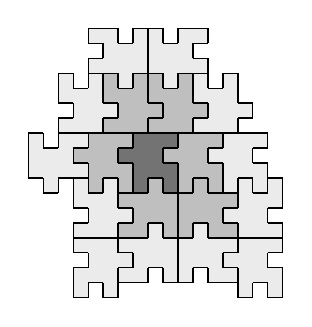
\begin{tikzpicture}[x=0.19cm,y=0.19cm,line width=0.5pt]
\fill[black!8] (-6,1) rectangle +(1,1);
\fill[black!8] (-6,2) rectangle +(1,1);
\fill[black!8] (-6,3) rectangle +(1,1);
\fill[black!8] (-5,0) rectangle +(1,1);
\fill[black!8] (-5,1) rectangle +(1,1);
\fill[black!8] (-5,2) rectangle +(1,1);
\fill[black!8] (-4,1) rectangle +(1,1);
\fill[black!8] (-4,2) rectangle +(1,1);
\fill[black!8] (-4,3) rectangle +(1,1);
\fill[black!8] (-4,4) rectangle +(1,1);
\fill[black!8] (-4,6) rectangle +(1,1);
\fill[black!8] (-4,7) rectangle +(1,1);
\fill[black!8] (-3,-7) rectangle +(1,1);
\fill[black!8] (-3,-6) rectangle +(1,1);
\fill[black!8] (-3,-4) rectangle +(1,1);
\fill[black!8] (-3,-3) rectangle +(1,1);
\fill[black!8] (-3,-1) rectangle +(1,1);
\fill[black!8] (-3,0) rectangle +(1,1);
\fill[black!8] (-3,1) rectangle +(1,1);
\fill[black!25] (-3,2) rectangle +(1,1);
\fill[black!8] (-3,3) rectangle +(1,1);
\fill[black!8] (-3,4) rectangle +(1,1);
\fill[black!8] (-3,5) rectangle +(1,1);
\fill[black!8] (-3,6) rectangle +(1,1);
\fill[black!8] (-2,-6) rectangle +(1,1);
\fill[black!8] (-2,-5) rectangle +(1,1);
\fill[black!8] (-2,-4) rectangle +(1,1);
\fill[black!8] (-2,-3) rectangle +(1,1);
\fill[black!8] (-2,-2) rectangle +(1,1);
\fill[black!8] (-2,-1) rectangle +(1,1);
\fill[black!25] (-2,0) rectangle +(1,1);
\fill[black!25] (-2,1) rectangle +(1,1);
\fill[black!25] (-2,2) rectangle +(1,1);
\fill[black!25] (-2,3) rectangle +(1,1);
\fill[black!8] (-2,4) rectangle +(1,1);
\fill[black!8] (-2,5) rectangle +(1,1);
\fill[black!8] (-2,6) rectangle +(1,1);
\fill[black!8] (-2,7) rectangle +(1,1);
\fill[black!8] (-2,8) rectangle +(1,1);
\fill[black!8] (-2,10) rectangle +(1,1);
\fill[black!8] (-1,-7) rectangle +(1,1);
\fill[black!8] (-1,-6) rectangle +(1,1);
\fill[black!8] (-1,-5) rectangle +(1,1);
\fill[black!8] (-1,-4) rectangle +(1,1);
\fill[black!8] (-1,-3) rectangle +(1,1);
\fill[black!8] (-1,-2) rectangle +(1,1);
\fill[black!8] (-1,-1) rectangle +(1,1);
\fill[black!8] (-1,0) rectangle +(1,1);
\fill[black!25] (-1,1) rectangle +(1,1);
\fill[black!25] (-1,2) rectangle +(1,1);
\fill[black!25] (-1,3) rectangle +(1,1);
\fill[black!25] (-1,4) rectangle +(1,1);
\fill[black!8] (-1,5) rectangle +(1,1);
\fill[black!25] (-1,6) rectangle +(1,1);
\fill[black!25] (-1,7) rectangle +(1,1);
\fill[black!8] (-1,8) rectangle +(1,1);
\fill[black!8] (-1,9) rectangle +(1,1);
\fill[black!8] (-1,10) rectangle +(1,1);
\fill[black!8] (0,-6) rectangle +(1,1);
\fill[black!8] (0,-5) rectangle +(1,1);
\fill[black!8] (0,-4) rectangle +(1,1);
\fill[black!25] (0,-3) rectangle +(1,1);
\fill[black!8] (0,-2) rectangle +(1,1);
\fill[black!25] (0,-1) rectangle +(1,1);
\fill[black!25] (0,0) rectangle +(1,1);
\fill[black!25] (0,1) rectangle +(1,1);
\fill[black!55] (0,2) rectangle +(1,1);
\fill[black!25] (0,3) rectangle +(1,1);
\fill[black!25] (0,4) rectangle +(1,1);
\fill[black!25] (0,5) rectangle +(1,1);
\fill[black!25] (0,6) rectangle +(1,1);
\fill[black!8] (0,7) rectangle +(1,1);
\fill[black!8] (0,8) rectangle +(1,1);
\fill[black!8] (0,9) rectangle +(1,1);
\fill[black!8] (1,-6) rectangle +(1,1);
\fill[black!8] (1,-5) rectangle +(1,1);
\fill[black!8] (1,-4) rectangle +(1,1);
\fill[black!25] (1,-3) rectangle +(1,1);
\fill[black!25] (1,-2) rectangle +(1,1);
\fill[black!25] (1,-1) rectangle +(1,1);
\fill[black!55] (1,0) rectangle +(1,1);
\fill[black!55] (1,1) rectangle +(1,1);
\fill[black!55] (1,2) rectangle +(1,1);
\fill[black!55] (1,3) rectangle +(1,1);
\fill[black!25] (1,4) rectangle +(1,1);
\fill[black!25] (1,5) rectangle +(1,1);
\fill[black!25] (1,6) rectangle +(1,1);
\fill[black!25] (1,7) rectangle +(1,1);
\fill[black!8] (1,8) rectangle +(1,1);
\fill[black!8] (1,9) rectangle +(1,1);
\fill[black!8] (1,10) rectangle +(1,1);
\fill[black!8] (2,-5) rectangle +(1,1);
\fill[black!8] (2,-4) rectangle +(1,1);
\fill[black!8] (2,-3) rectangle +(1,1);
\fill[black!25] (2,-2) rectangle +(1,1);
\fill[black!25] (2,-1) rectangle +(1,1);
\fill[black!25] (2,0) rectangle +(1,1);
\fill[black!55] (2,1) rectangle +(1,1);
\fill[black!55] (2,2) rectangle +(1,1);
\fill[black!55] (2,3) rectangle +(1,1);
\fill[black!25] (2,4) rectangle +(1,1);
\fill[black!25] (2,5) rectangle +(1,1);
\fill[black!25] (2,6) rectangle +(1,1);
\fill[black!25] (2,7) rectangle +(1,1);
\fill[black!8] (2,8) rectangle +(1,1);
\fill[black!8] (2,9) rectangle +(1,1);
\fill[black!8] (2,10) rectangle +(1,1);
\fill[black!8] (3,-6) rectangle +(1,1);
\fill[black!8] (3,-5) rectangle +(1,1);
\fill[black!8] (3,-4) rectangle +(1,1);
\fill[black!25] (3,-3) rectangle +(1,1);
\fill[black!25] (3,-2) rectangle +(1,1);
\fill[black!25] (3,-1) rectangle +(1,1);
\fill[black!55] (3,0) rectangle +(1,1);
\fill[black!55] (3,1) rectangle +(1,1);
\fill[black!25] (3,2) rectangle +(1,1);
\fill[black!55] (3,3) rectangle +(1,1);
\fill[black!25] (3,4) rectangle +(1,1);
\fill[black!25] (3,5) rectangle +(1,1);
\fill[black!25] (3,6) rectangle +(1,1);
\fill[black!8] (3,7) rectangle +(1,1);
\fill[black!8] (3,8) rectangle +(1,1);
\fill[black!8] (3,9) rectangle +(1,1);
\fill[black!8] (4,-6) rectangle +(1,1);
\fill[black!8] (4,-5) rectangle +(1,1);
\fill[black!8] (4,-4) rectangle +(1,1);
\fill[black!25] (4,-3) rectangle +(1,1);
\fill[black!25] (4,-2) rectangle +(1,1);
\fill[black!25] (4,-1) rectangle +(1,1);
\fill[black!25] (4,0) rectangle +(1,1);
\fill[black!25] (4,1) rectangle +(1,1);
\fill[black!25] (4,2) rectangle +(1,1);
\fill[black!25] (4,3) rectangle +(1,1);
\fill[black!25] (4,4) rectangle +(1,1);
\fill[black!25] (4,5) rectangle +(1,1);
\fill[black!25] (4,6) rectangle +(1,1);
\fill[black!25] (4,7) rectangle +(1,1);
\fill[black!8] (4,8) rectangle +(1,1);
\fill[black!8] (4,9) rectangle +(1,1);
\fill[black!8] (4,10) rectangle +(1,1);
\fill[black!8] (5,-5) rectangle +(1,1);
\fill[black!8] (5,-4) rectangle +(1,1);
\fill[black!8] (5,-3) rectangle +(1,1);
\fill[black!25] (5,-2) rectangle +(1,1);
\fill[black!25] (5,-1) rectangle +(1,1);
\fill[black!25] (5,0) rectangle +(1,1);
\fill[black!25] (5,1) rectangle +(1,1);
\fill[black!25] (5,2) rectangle +(1,1);
\fill[black!25] (5,3) rectangle +(1,1);
\fill[black!8] (5,4) rectangle +(1,1);
\fill[black!25] (5,5) rectangle +(1,1);
\fill[black!8] (5,6) rectangle +(1,1);
\fill[black!8] (5,7) rectangle +(1,1);
\fill[black!8] (5,8) rectangle +(1,1);
\fill[black!8] (5,10) rectangle +(1,1);
\fill[black!8] (6,-6) rectangle +(1,1);
\fill[black!8] (6,-5) rectangle +(1,1);
\fill[black!8] (6,-4) rectangle +(1,1);
\fill[black!25] (6,-3) rectangle +(1,1);
\fill[black!25] (6,-2) rectangle +(1,1);
\fill[black!25] (6,-1) rectangle +(1,1);
\fill[black!25] (6,0) rectangle +(1,1);
\fill[black!25] (6,1) rectangle +(1,1);
\fill[black!8] (6,2) rectangle +(1,1);
\fill[black!25] (6,3) rectangle +(1,1);
\fill[black!8] (6,4) rectangle +(1,1);
\fill[black!8] (6,5) rectangle +(1,1);
\fill[black!8] (6,6) rectangle +(1,1);
\fill[black!8] (7,-6) rectangle +(1,1);
\fill[black!8] (7,-5) rectangle +(1,1);
\fill[black!8] (7,-4) rectangle +(1,1);
\fill[black!25] (7,-3) rectangle +(1,1);
\fill[black!8] (7,-2) rectangle +(1,1);
\fill[black!25] (7,-1) rectangle +(1,1);
\fill[black!8] (7,0) rectangle +(1,1);
\fill[black!8] (7,1) rectangle +(1,1);
\fill[black!8] (7,2) rectangle +(1,1);
\fill[black!8] (7,3) rectangle +(1,1);
\fill[black!8] (7,4) rectangle +(1,1);
\fill[black!8] (7,5) rectangle +(1,1);
\fill[black!8] (7,6) rectangle +(1,1);
\fill[black!8] (7,7) rectangle +(1,1);
\fill[black!8] (8,-7) rectangle +(1,1);
\fill[black!8] (8,-6) rectangle +(1,1);
\fill[black!8] (8,-5) rectangle +(1,1);
\fill[black!8] (8,-4) rectangle +(1,1);
\fill[black!8] (8,-3) rectangle +(1,1);
\fill[black!8] (8,-2) rectangle +(1,1);
\fill[black!8] (8,-1) rectangle +(1,1);
\fill[black!8] (8,0) rectangle +(1,1);
\fill[black!8] (8,1) rectangle +(1,1);
\fill[black!8] (8,2) rectangle +(1,1);
\fill[black!8] (8,3) rectangle +(1,1);
\fill[black!8] (8,5) rectangle +(1,1);
\fill[black!8] (9,-6) rectangle +(1,1);
\fill[black!8] (9,-5) rectangle +(1,1);
\fill[black!8] (9,-4) rectangle +(1,1);
\fill[black!8] (9,-3) rectangle +(1,1);
\fill[black!8] (9,-2) rectangle +(1,1);
\fill[black!8] (9,-1) rectangle +(1,1);
\fill[black!8] (9,0) rectangle +(1,1);
\fill[black!8] (9,1) rectangle +(1,1);
\fill[black!8] (9,3) rectangle +(1,1);
\fill[black!8] (10,-7) rectangle +(1,1);
\fill[black!8] (10,-6) rectangle +(1,1);
\fill[black!8] (10,-4) rectangle +(1,1);
\fill[black!8] (10,-3) rectangle +(1,1);
\fill[black!8] (10,-1) rectangle +(1,1);
\fill[black!8] (10,0) rectangle +(1,1);
\draw (-6,1)--(-6,2);
\draw (-6,1)--(-5,1);
\draw (-6,2)--(-6,3);
\draw (-6,3)--(-6,4);
\draw (-6,4)--(-5,4);
\draw (-5,0)--(-5,1);
\draw (-5,0)--(-4,0);
\draw (-5,3)--(-5,4);
\draw (-5,3)--(-4,3);
\draw (-4,0)--(-4,1);
\draw (-4,1)--(-3,1);
\draw (-4,3)--(-4,4);
\draw (-4,4)--(-4,5);
\draw (-4,4)--(-3,4);
\draw (-4,5)--(-3,5);
\draw (-4,6)--(-4,7);
\draw (-4,6)--(-3,6);
\draw (-4,7)--(-4,8);
\draw (-4,8)--(-3,8);
\draw (-3,-7)--(-3,-6);
\draw (-3,-7)--(-2,-7);
\draw (-3,-6)--(-3,-5);
\draw (-3,-5)--(-2,-5);
\draw (-3,-4)--(-3,-3);
\draw (-3,-4)--(-2,-4);
\draw (-3,-3)--(-3,-2);
\draw (-3,-3)--(-2,-3);
\draw (-3,-2)--(-2,-2);
\draw (-3,-1)--(-3,0);
\draw (-3,-1)--(-2,-1);
\draw (-3,0)--(-3,1);
\draw (-3,1)--(-2,1);
\draw (-3,2)--(-3,3);
\draw (-3,2)--(-2,2);
\draw (-3,3)--(-2,3);
\draw (-3,4)--(-2,4);
\draw (-3,5)--(-3,6);
\draw (-3,7)--(-3,8);
\draw (-3,7)--(-2,7);
\draw (-2,-7)--(-2,-6);
\draw (-2,-6)--(-1,-6);
\draw (-2,-5)--(-2,-4);
\draw (-2,-3)--(-1,-3);
\draw (-2,-2)--(-2,-1);
\draw (-2,0)--(-2,1);
\draw (-2,0)--(-1,0);
\draw (-2,1)--(-2,2);
\draw (-2,3)--(-2,4);
\draw (-2,4)--(-1,4);
\draw (-2,7)--(-2,8);
\draw (-2,8)--(-2,9);
\draw (-2,8)--(-1,8);
\draw (-2,9)--(-1,9);
\draw (-2,10)--(-2,11);
\draw (-2,10)--(-1,10);
\draw (-2,11)--(-1,11);
\draw (-1,-7)--(-1,-6);
\draw (-1,-7)--(0,-7);
\draw (-1,-3)--(0,-3);
\draw (-1,0)--(-1,1);
\draw (-1,1)--(0,1);
\draw (-1,4)--(-1,5);
\draw (-1,4)--(0,4);
\draw (-1,5)--(0,5);
\draw (-1,6)--(-1,7);
\draw (-1,6)--(0,6);
\draw (-1,7)--(-1,8);
\draw (-1,8)--(0,8);
\draw (-1,9)--(-1,10);
\draw (-1,11)--(0,11);
\draw (0,-7)--(0,-6);
\draw (0,-6)--(0,-5);
\draw (0,-6)--(1,-6);
\draw (0,-5)--(1,-5);
\draw (0,-4)--(0,-3);
\draw (0,-4)--(1,-4);
\draw (0,-3)--(0,-2);
\draw (0,-3)--(1,-3);
\draw (0,-2)--(1,-2);
\draw (0,-1)--(0,0);
\draw (0,-1)--(1,-1);
\draw (0,0)--(0,1);
\draw (0,0)--(1,0);
\draw (0,2)--(0,3);
\draw (0,2)--(1,2);
\draw (0,3)--(1,3);
\draw (0,4)--(1,4);
\draw (0,5)--(0,6);
\draw (0,7)--(0,8);
\draw (0,7)--(1,7);
\draw (0,10)--(0,11);
\draw (0,10)--(1,10);
\draw (1,-6)--(2,-6);
\draw (1,-5)--(1,-4);
\draw (1,-3)--(2,-3);
\draw (1,-2)--(1,-1);
\draw (1,0)--(1,1);
\draw (1,0)--(2,0);
\draw (1,1)--(1,2);
\draw (1,3)--(1,4);
\draw (1,4)--(2,4);
\draw (1,7)--(1,8);
\draw (1,8)--(2,8);
\draw (1,10)--(1,11);
\draw (1,11)--(2,11);
\draw (2,-6)--(2,-5);
\draw (2,-5)--(3,-5);
\draw (2,-3)--(2,-2);
\draw (2,-2)--(3,-2);
\draw (2,0)--(2,1);
\draw (2,1)--(3,1);
\draw (2,4)--(2,5);
\draw (2,4)--(3,4);
\draw (2,5)--(3,5);
\draw (2,6)--(2,7);
\draw (2,6)--(3,6);
\draw (2,7)--(2,8);
\draw (2,8)--(2,9);
\draw (2,8)--(3,8);
\draw (2,9)--(2,10);
\draw (2,10)--(2,11);
\draw (2,11)--(3,11);
\draw (3,-6)--(3,-5);
\draw (3,-6)--(4,-6);
\draw (3,-3)--(3,-2);
\draw (3,-3)--(4,-3);
\draw (3,0)--(3,1);
\draw (3,0)--(4,0);
\draw (3,2)--(3,3);
\draw (3,2)--(4,2);
\draw (3,3)--(4,3);
\draw (3,4)--(4,4);
\draw (3,5)--(3,6);
\draw (3,7)--(3,8);
\draw (3,7)--(4,7);
\draw (3,10)--(3,11);
\draw (3,10)--(4,10);
\draw (4,-6)--(4,-5);
\draw (4,-6)--(5,-6);
\draw (4,-5)--(4,-4);
\draw (4,-4)--(4,-3);
\draw (4,-3)--(4,-2);
\draw (4,-3)--(5,-3);
\draw (4,-2)--(4,-1);
\draw (4,-1)--(4,0);
\draw (4,0)--(4,1);
\draw (4,0)--(5,0);
\draw (4,1)--(4,2);
\draw (4,3)--(4,4);
\draw (4,4)--(5,4);
\draw (4,7)--(4,8);
\draw (4,8)--(5,8);
\draw (4,10)--(4,11);
\draw (4,11)--(5,11);
\draw (5,-6)--(5,-5);
\draw (5,-5)--(6,-5);
\draw (5,-3)--(5,-2);
\draw (5,-2)--(6,-2);
\draw (5,0)--(5,1);
\draw (5,1)--(6,1);
\draw (5,4)--(5,5);
\draw (5,4)--(6,4);
\draw (5,5)--(6,5);
\draw (5,6)--(5,7);
\draw (5,6)--(6,6);
\draw (5,7)--(5,8);
\draw (5,8)--(6,8);
\draw (5,9)--(5,10);
\draw (5,9)--(6,9);
\draw (5,10)--(6,10);
\draw (5,11)--(6,11);
\draw (6,-6)--(6,-5);
\draw (6,-6)--(7,-6);
\draw (6,-3)--(6,-2);
\draw (6,-3)--(7,-3);
\draw (6,0)--(6,1);
\draw (6,0)--(7,0);
\draw (6,2)--(6,3);
\draw (6,2)--(7,2);
\draw (6,3)--(7,3);
\draw (6,4)--(7,4);
\draw (6,5)--(6,6);
\draw (6,7)--(6,8);
\draw (6,7)--(7,7);
\draw (6,8)--(6,9);
\draw (6,10)--(6,11);
\draw (7,-6)--(8,-6);
\draw (7,-5)--(7,-4);
\draw (7,-5)--(8,-5);
\draw (7,-4)--(8,-4);
\draw (7,-3)--(8,-3);
\draw (7,-2)--(7,-1);
\draw (7,-2)--(8,-2);
\draw (7,-1)--(8,-1);
\draw (7,0)--(7,1);
\draw (7,0)--(8,0);
\draw (7,1)--(7,2);
\draw (7,3)--(7,4);
\draw (7,4)--(8,4);
\draw (7,7)--(7,8);
\draw (7,8)--(8,8);
\draw (8,-7)--(8,-6);
\draw (8,-7)--(9,-7);
\draw (8,-6)--(8,-5);
\draw (8,-4)--(8,-3);
\draw (8,-3)--(8,-2);
\draw (8,-3)--(9,-3);
\draw (8,-1)--(8,0);
\draw (8,0)--(8,1);
\draw (8,1)--(9,1);
\draw (8,4)--(8,5);
\draw (8,4)--(9,4);
\draw (8,5)--(9,5);
\draw (8,6)--(8,7);
\draw (8,6)--(9,6);
\draw (8,7)--(8,8);
\draw (9,-7)--(9,-6);
\draw (9,-6)--(10,-6);
\draw (9,-3)--(10,-3);
\draw (9,0)--(9,1);
\draw (9,0)--(10,0);
\draw (9,2)--(9,3);
\draw (9,2)--(10,2);
\draw (9,3)--(10,3);
\draw (9,4)--(10,4);
\draw (9,5)--(9,6);
\draw (10,-7)--(10,-6);
\draw (10,-7)--(11,-7);
\draw (10,-5)--(10,-4);
\draw (10,-5)--(11,-5);
\draw (10,-4)--(11,-4);
\draw (10,-3)--(11,-3);
\draw (10,-2)--(10,-1);
\draw (10,-2)--(11,-2);
\draw (10,-1)--(11,-1);
\draw (10,0)--(10,1);
\draw (10,1)--(10,2);
\draw (10,1)--(11,1);
\draw (10,3)--(10,4);
\draw (11,-7)--(11,-6);
\draw (11,-6)--(11,-5);
\draw (11,-4)--(11,-3);
\draw (11,-3)--(11,-2);
\draw (11,-1)--(11,0);
\draw (11,0)--(11,1);
\end{tikzpicture}
\caption{The unique inner part of 11-omino \#2 ($k=\Hh=3$), drawn from the
recorded cell coordinates: the central shape (dark), its six copies of
layer~1 (medium) and twelve copies of layer~2 (light). Both
implementations record exactly this configuration. It has 1,250 outer
completions.}
\label{fig:inner}
\end{figure}

\subsection{Comparison with public enumeration reports}
Enumerating coronas and studying forced configurations have clear
precedents. Kaplan's heesch-sat software~\cite{heeschsat} enumerates the
one-layer surrounds of a shape, separating those with and without holes,
and contains a routine that counts hole-free coronas by successively
excluding SAT solutions. Mann~\cite{Mann} discusses generating all first
and second coronas of a shape. Kaplan~\cite[p.~170 of the journal
version]{Kaplan} points to the forced groupings of tiles described by
Mann and Thomas~\cite{MannThomas}. Public reports of the Heesch
challenge~\cite{LayrReports} enumerate coronas of several shapes counted
here. To compare like quantities, separate calculations with the first
implementation count all one- and two-layer $\Hc$-coronas, without
requiring extension to four layers; each enumeration ends with a
drat-trim-checked unsatisfiable call, and these counts were not repeated
by the second implementation.
For 16-hex \#2 the counts 251 and 1,449 match discussion~\#32; the
unique second-layer prefix extendable to four layers also matches the
reported count. For 11-hex \#18 the one-layer count 793 matches
\#12. Shape coordinates have not been compared with those reports,
so equal reported counts are not treated as a proof of input identity.

Discussion~\#94 reports 1,027 complete four-layer patches of the
20-iamond, whereas our $\Hc$ count is 2,418,624. Its counted object,
equivalence relation and treatment of unfinished branches have not been
aligned with ours. The discrepancy therefore does not identify an error
on either side. We provide counts under the explicit conventions above,
without a priority claim for counting coronas.

\section{A restricted search for finite-\texorpdfstring{$\Hh=4$}{Hh=4} polyominoes}
\label{sec:search}
Kaplan's published search through 19 cells gives largest finite $\Hh=3$
for unmarked polyominoes~\cite{Kaplan}. We examine a fixed collection of
3,442 hole-free, edge-connected polyominoes with 20--28 cells. Candidates
are normalized under translation, rotation and reflection and arise from
five biased construction families: anisotropic integer enlargement of
the five polyominoes with $\Hh=3$ in Table~\ref{tab:values} (4);
repeating one row or column of one of these five shapes one to three
times (82); two successive such repetitions (1,223); cell additions to
the same five shapes until 20 cells (612); and one-cell additions to the
767 shapes of Kaplan's file \texttt{19omino\_2up} (1,521). That file
lists the 19-cell polyominoes with $\Hh\geq2$, all of which have
$\Hh=2$; it is not a list of all 19-cell polyominoes.
Duplicates are assigned to the earliest family. The final family selects
at most two shapes per parent in a fixed hash order from 17,302 generated
free shapes; the full generated family is not screened.

The screening tests $K=3$ for $\Hh$, with a $K=1$ pretest for part of
the collection. By Lemma~\ref{lem:trunc}, either UNSAT result excludes
$\Hh=4$. Satisfying patches are checked geometrically. Explicit periodic
tilings are then sought before deeper SAT tests. A tiling certificate
places congruent copies in an integer-lattice fundamental domain and
checks complete coverage and non-overlap, including all translates.
The retained outcomes are in Table~\ref{tab:search}. The two UNSAT
columns describe the actual screening stages, not exact Heesch values.

\begin{table}[!htbp]
\centering\small
\begin{tabular}{@{}rrrrr@{}}
\toprule
Cells & $K=1$ UNSAT & $K=3$ UNSAT & Periodic tiling & Total\\
\midrule
20 & 962 & 770 & 488 & 2,220\\
21 & 38 & 56 & 11 & 105\\
22 & 53 & 85 & 10 & 148\\
23 & 76 & 102 & 4 & 182\\
24 & 57 & 57 & 22 & 136\\
25 & 107 & 95 & 8 & 210\\
26 & 70 & 69 & 15 & 154\\
27 & 90 & 65 & 10 & 165\\
28 & 62 & 52 & 8 & 122\\
\midrule
Total & 1,515 & 1,351 & 576 & 3,442\\
\bottomrule
\end{tabular}
\caption{Outcomes on the restricted collection. There are no unprocessed
or undecided candidates in this collection. The periodic tilings use
one (65 shapes), two (413) or four (98) copies per fundamental domain.}
\label{tab:search}
\end{table}

Of 1,862 shapes actually tested at $K=3$, 511 are satisfiable and all
511 have explicit periodic tilings; 65 further shapes are eliminated by
one-copy periodic tilings. One 20-cell shape tested at $K=4$ is also
satisfiable at $K=5$ and has a four-copy periodic tiling with lattice
basis $(40,0),(18,2)$. Its four-layer patch is consequently not evidence
of a finite value four.

A separate finite audit checks the candidate identities, topology and
all 576 periodic tilings. Fourteen UNSAT instances agree with a second
SAT solver using the same encoding; two representative screening
instances have drat-trim-accepted proofs. The remaining UNSAT outcomes
are solver records without proof logs. All 513 saved satisfying patches
(511 at $K=3$, one at $K=4$ and one at $K=5$) pass geometric checking.
These checks yield no finite-$\Hh=4$ example. They do not establish
that such a polyomino is impossible: the collection is neither an
exhaustive size census nor a random sample.

\section{Scope and remarks}
\label{sec:scope}
\paragraph{What the certificates do not cover.}
The values are certified for the listed shapes only. That Kaplan's files
contain every non-tiler of each size is taken from his enumeration and is
not checked here. Polyominoes with 11--19 cells and $\Hh\leq2$, polyhexes
with 9--16 cells and $\Hh\leq3$, polyhexes with 17 or more cells, and
polyiamonds with 13--24 cells and $\Hh\leq3$ are outside the selection.
All statements concern copies on the fixed grid; a statement about
arbitrary placements in the plane would need a further reduction.

\paragraph{Relation to other certification work.}
The Heesch challenge~\cite{Layr} provides, for individual shapes, a
route through LRAT to the verified checker cake\_lpr~\cite{cakelpr};
here every proof is checked by drat-trim, which is not formally verified, but the
correspondence between geometry and CNF is a Lean theorem, and the
correspondence between that theorem and the checked files is a recorded
finite comparison. The empty hexagon verification~\cite{EmptyHex}
connects its Lean reduction to the external cake\_lpr result through an
explicit axiom; Szeider~\cite{Szeider} streams LRAT certificates into Lean
theorems, with native evaluation in the trusted base; and bv\_decide
\cite{Boving} uses verified bit-blasting and LRAT checking inside Lean.
Converting the 5,019 proofs to LRAT~\cite{LRAT} and checking them with
a verified checker, or inside Lean, would remove drat-trim from the trusted
base; replacing the file comparison by a Lean proof about the generating
program would remove the transcription. Neither has been done.

\paragraph{Novelty.}
A literature search of published papers, preprints and public code up to
22 October 2026 found certificates for individual Heesch numbers
\cite{Layr} and Lean-verified reductions from combinatorial or geometric
problems to SAT \cite{CAH,Holliday,EmptyHex}, but not the combination
reported here: a fixed table range with witnesses, proofs and a second
encoding for every value, and a Lean soundness theorem for a Heesch
encoding on three grids connected to the checked files. Public corona
enumeration reports~\cite{LayrReports} overlap the counting questions;
Section~\ref{sec:counts} compares their values under explicit counting
conventions. The restricted search is a record of the tested collection,
not a new extremal construction. The search was
not exhaustive, and we claim no priority beyond it.

\paragraph{Records.}
The following records accompany this article: the witnesses; the
certificate records with the hashes of every CNF and proof; the Lean
sources; the records of the file comparison; for the counts of
Section~\ref{sec:counts}, the cell coordinates of every enumerated inner
part from both implementations, the per-inner-part outer completion
counts, and the hashes and drat-trim results of the enumeration proofs;
and for the search of Section~\ref{sec:search}, the candidate list with
its SHA-256 hash, the classification of every candidate, the periodic
tiling certificates and the saved satisfying patches.

\section*{AI-use statement}
AI systems assisted with the computation of the values, witnesses and
proofs, the second encoding and the geometric checkers, the Lean
statement and proof, the independent reading of the Lean statement, the
file comparison, maximal-corona enumeration and counting, candidate
generation and screening, literature organization and manuscript drafting. The
author is responsible for the claims and their stated scope; AI systems
are not authors.

{\raggedright\small
\begin{thebibliography}{99}
\bibitem{Basic21}
B. Ba\v{s}i\'c,
``A figure with Heesch number 6: pushing a two-decade-old boundary,''
\emph{Math. Intelligencer} \textbf{43}(3), 50--53 (2021),
\href{https://doi.org/10.1007/s00283-020-10034-w}{doi:10.1007/s00283-020-10034-w}.

\bibitem{Basic26}
B. Ba\v{s}i\'c,
``The Heesch number in $\mathbb E^3$ is unbounded,''
\href{https://arxiv.org/abs/2610.24281v1}{arXiv:2610.24281v1} (2026).

\bibitem{Boving}
H. Böving et al.,
``Interactive bitvector reasoning using verified bit-blasting,''
\emph{Proc. ACM Program. Lang.} \textbf{9}(OOPSLA2), 3259--3285 (2025),
\href{https://doi.org/10.1145/3763167}{doi:10.1145/3763167}.

\bibitem{CodelThesis}
C. R. Codel,
\emph{Verifying SAT Encodings in Lean},
M.S. thesis, Carnegie Mellon University (2022),
\url{https://crcodel.com/research/verified_encodings_thesis.pdf}.

\bibitem{CAH}
C. R. Codel, J. Avigad and M. J. H. Heule,
``Verified encodings for SAT solvers,''
in \emph{Proc. FMCAD 2023}, 141--151,
\href{https://doi.org/10.34727/2023/isbn.978-3-85448-060-0_22}{doi:10.34727/2023/isbn.978-3-85448-060-0\_22}.

\bibitem{LRAT}
L. Cruz-Filipe, M. J. H. Heule, W. A. Hunt Jr., M. Kaufmann and
P. Schneider-Kamp,
``Efficient certified RAT verification,''
in \emph{CADE-26}, LNCS \textbf{10395}, 220--236 (2017),
\href{https://doi.org/10.1007/978-3-319-63046-5_14}{doi:10.1007/978-3-319-63046-5\_14}.

\bibitem{Fontaine}
A. Fontaine,
``An infinite number of plane figures with Heesch number two,''
\emph{J. Combin. Theory Ser. A} \textbf{57}(1), 151--156 (1991),
\href{https://doi.org/10.1016/0097-3165(91)90013-7}{doi:10.1016/0097-3165(91)90013-7}.

\bibitem{Heesch}
H. Heesch,
\emph{Reguläres Parkettierungsproblem},
Westdeutscher Verlag, Köln/Opladen (1968),
\href{https://doi.org/10.1007/978-3-322-98547-7}{doi:10.1007/978-3-322-98547-7}.

\bibitem{Holliday}
W. H. Holliday, C. Norman, E. Pacuit and S. Zahedian,
``Impossibility theorems involving weakenings of expansion consistency
and resoluteness in voting,''
\href{https://arxiv.org/abs/2208.06907v3}{arXiv:2208.06907v3} (2023),
Appendix~C.

\bibitem{Kaplan}
C. S. Kaplan,
``Heesch numbers of unmarked polyforms,''
\emph{Contrib. Discrete Math.} \textbf{17}(2), 150--171 (2022),
\href{https://doi.org/10.55016/ojs/cdm.v17i2.72886}{doi:10.55016/ojs/cdm.v17i2.72886};
\href{https://arxiv.org/abs/2105.09438v1}{arXiv:2105.09438v1} (2021);
data at \url{https://cs.uwaterloo.ca/~csk/heesch/}.
Section numbers refer to arXiv:2105.09438v1.

\bibitem{Kaplan25}
C. S. Kaplan,
``The path to aperiodic monotiles,''
\href{https://arxiv.org/abs/2509.12216v1}{arXiv:2509.12216v1} (2025).

\bibitem{heeschsat}
isohedral/heesch-sat contributors,
\emph{heesch-sat}, software,
\url{https://github.com/isohedral/heesch-sat},
commit \nolinkurl{d12a527c04310fed51d522318126781e2f7ed56d}.

\bibitem{Layr}
Layr-Labs/Eigen and contributors,
\emph{Heesch challenge}, software and specifications,
\url{https://github.com/Layr-Labs/heesch},
commit \nolinkurl{947f05720e0842d80b5119b9b88546c890111d19}.

\bibitem{Maiti}
A. Maiti,
``Unboundedness of the Heesch number for hyperbolic convex monotiles,''
\href{https://arxiv.org/abs/2603.27827v3}{arXiv:2603.27827v3} (2026).

\bibitem{Mann}
C. Mann,
``Heesch's tiling problem,''
\emph{Amer. Math. Monthly} \textbf{111}(6), 509--517 (2004),
\href{https://doi.org/10.1080/00029890.2004.11920105}{doi:10.1080/00029890.2004.11920105}.

\bibitem{MannThomas}
C. Mann and B. C. Thomas,
``Heesch numbers of edge-marked polyforms,''
\emph{Exp. Math.} \textbf{25}(3), 281--294 (2016),
\href{https://doi.org/10.1080/10586458.2015.1096867}{doi:10.1080/10586458.2015.1096867}.

\bibitem{Sinz}
C. Sinz,
``Towards an optimal CNF encoding of Boolean cardinality constraints,''
in \emph{CP 2005}, LNCS \textbf{3709}, 827--831,
\href{https://doi.org/10.1007/11564751_73}{doi:10.1007/11564751\_73}.

\bibitem{EmptyHex}
B. Subercaseaux, W. Nawrocki, J. Gallicchio, C. Codel, M. Carneiro and
M. J. H. Heule,
``Formal verification of the empty hexagon number,''
in \emph{ITP 2024}, LIPIcs \textbf{309}, 35:1--35:19,
\href{https://doi.org/10.4230/LIPIcs.ITP.2024.35}{doi:10.4230/LIPIcs.ITP.2024.35}.

\bibitem{Szeider}
S. Szeider,
``Streaming LRAT certificates into Lean theorems,''
\href{https://arxiv.org/abs/2607.00815v2}{arXiv:2607.00815v2} (2026).

\bibitem{cakelpr}
Y. K. Tan, M. J. H. Heule and M. O. Myreen,
``cake\_lpr: verified propagation redundancy checking in CakeML,''
in \emph{TACAS 2021}, LNCS \textbf{12652}, 223--241,
\href{https://doi.org/10.1007/978-3-030-72013-1_12}{doi:10.1007/978-3-030-72013-1\_12}.

\bibitem{dratTrim}
N. Wetzler, M. J. H. Heule and W. A. Hunt Jr.,
``DRAT-trim: efficient checking and trimming using expressive clausal
proofs,''
in \emph{SAT 2014}, LNCS \textbf{8561}, 422--429,
\href{https://doi.org/10.1007/978-3-319-09284-3_31}{doi:10.1007/978-3-319-09284-3\_31}.

\bibitem{Lean4}
L. de Moura and S. Ullrich,
``The Lean 4 theorem prover and programming language,''
in \emph{CADE 28}, LNCS \textbf{12699}, 625--635 (2021),
\href{https://doi.org/10.1007/978-3-030-79876-5_37}{doi:10.1007/978-3-030-79876-5\_37}.

\bibitem{Mathlib}
The mathlib Community,
``The Lean mathematical library,''
in \emph{CPP 2020}, 367--381,
\href{https://doi.org/10.1145/3372885.3373824}{doi:10.1145/3372885.3373824};
Lean 4 library: \url{https://github.com/leanprover-community/mathlib4}.

\bibitem{Comparator}
Lean project contributors,
\emph{Comparator}, software,
\url{https://github.com/leanprover/comparator}.

\bibitem{Lean4Lean}
M. Carneiro,
``Lean4Lean: verifying a typechecker for Lean, in Lean,''
\href{https://arxiv.org/abs/2403.14064v3}{arXiv:2403.14064v3} (2025);
software: \url{https://github.com/digama0/lean4lean}.

\bibitem{OtherKernels}
Nanoda, ConLeche and ConRon contributors,
external Lean checker software:
\url{https://github.com/ammkrn/nanoda_lib},
\url{https://github.com/leanprover/con-leche},
\url{https://github.com/leanprover/con-ron}.

\bibitem{PySAT}
A. Ignatiev, A. Morgado and J. Marques-Silva,
``PySAT: a Python toolkit for prototyping with SAT oracles,''
in \emph{SAT 2018}, LNCS \textbf{10929}, 428--437,
\href{https://doi.org/10.1007/978-3-319-94144-8_26}{doi:10.1007/978-3-319-94144-8\_26}.

\bibitem{CaDiCaL}
A. Biere and contributors,
\emph{CaDiCaL}, SAT solver software,
\url{https://github.com/arminbiere/cadical}.

\bibitem{Glucose}
G. Audemard and L. Simon,
\emph{Glucose}, SAT solver software,
\url{https://www.cril.univ-artois.fr/software/glucose/}.

\bibitem{Lingeling}
A. Biere,
\emph{Lingeling}, SAT solver software,
\url{https://github.com/arminbiere/lingeling}.

\bibitem{LayrReports}
Contributors to the Layr-Labs Heesch discussions,
public enumeration reports, discussions
\href{https://github.com/Layr-Labs/heesch/discussions/12}{\#12},
\href{https://github.com/Layr-Labs/heesch/discussions/32}{\#32} and
\href{https://github.com/Layr-Labs/heesch/discussions/94}{\#94}
(2026).
\end{thebibliography}
}
\end{document}
